\documentclass[10pt,xcolor=svgnames]{beamer} %Beamer


\usepackage{palatino} %font type
\usepackage{xcolor}
\usepackage[font={small}]{caption}
\usefonttheme{metropolis} %Type of slides
\usefonttheme[onlymath]{serif} %font type Mathematical expressions
\usetheme[progressbar=frametitle,titleformat frame=smallcaps,numbering=counter]{metropolis} %This adds a bar at the beginning of each section.
\useoutertheme[subsection=false]{miniframes} %Circles in the top of each frame, showing the slide of each section you are at

\usepackage{appendixnumberbeamer} %enumerate each slide without counting the appendix

\definecolor{SysBlue}{RGB}{12,120,183}
\definecolor{Progress}{RGB}{56,60,92}
\definecolor{Header}{RGB}{12,120,183}
\definecolor{SlideTitle}{RGB}{0,137,208}
\definecolor{ToC}{RGB}{51,58,66}

\setbeamercolor{progress bar}{fg=Progress} %These are the colours of the progress bar. Notice that the names used are the svgnames
\setbeamercolor{title separator}{fg=SysBlue} %This is the line colour in the title slide
\setbeamercolor{structure}{fg=black} %Colour of the text of structure, numbers, items, blah. Not the big text.
\setbeamercolor{normal text}{fg=black!87} %Colour of normal text
\setbeamercolor{alerted text}{fg=DarkRed!60!Gainsboro} %Color of the alert box
\setbeamercolor{example text}{fg=ToC} %Colour of the Example block text
\setbeamercolor{background canvas}{bg=white}


\setbeamercolor{palette primary}{bg=SlideTitle, fg=white} %These are the colours of the background. Being this the main combination and so one. 
\setbeamercolor{palette secondary}{bg=Header, fg=white}
\setbeamercolor{palette tertiary}{bg=Header, fg=white}
\setbeamercolor{section in toc}{fg=ToC} %Color of the text in the table of contents (toc)

\setbeamertemplate{blocks}[rounded][shadow=true]


%These next packages are the useful for Physics in general, you can add the extras here. 
\usepackage{amsmath,amssymb}
\usepackage{slashed}
\usepackage{cite}
\usepackage{relsize}
\usepackage{caption}
\usepackage{subcaption}
\usepackage{multicol}
\usepackage{booktabs}
\usepackage[scale=2]{ccicons}
\usepackage{pgfplots}
\usepgfplotslibrary{dateplot}
\usepackage{geometry}
\usepackage{xspace}

\newcommand{\themename}{\textbf{\textsc{bluetemp}\xspace}}%metropolis}}\xspace}

\title{Pachira Fund}
\author[Name]{Ian Moore, PhD \inst{$\dagger$}}%With inst, you can change the institution they belong
\subtitle{Pachira pitch video draft}

\institute[shortinst]{\inst{$\dagger$} Tokenomics Researcher / Engineer @ Syslabs (email: imoore@syscoin.org) }

\titlegraphic{\vspace{-0.5cm}\hfill
\includegraphics[scale=0.23]{logo.png}} %You can modify the location of the logo by changing the command \vspace{}. 

\begin{document}
{
\setbeamercolor{background canvas}{bg=white, fg=black}
\setbeamercolor{normal text}{fg=black}
\maketitle
}%This is the colour of the first slide. bg= background and fg=foreground

\metroset{titleformat frame=smallcaps} %This changes the titles for small caps


\begin{frame}{Video: Slide 1}
\begin{figure}[h!]
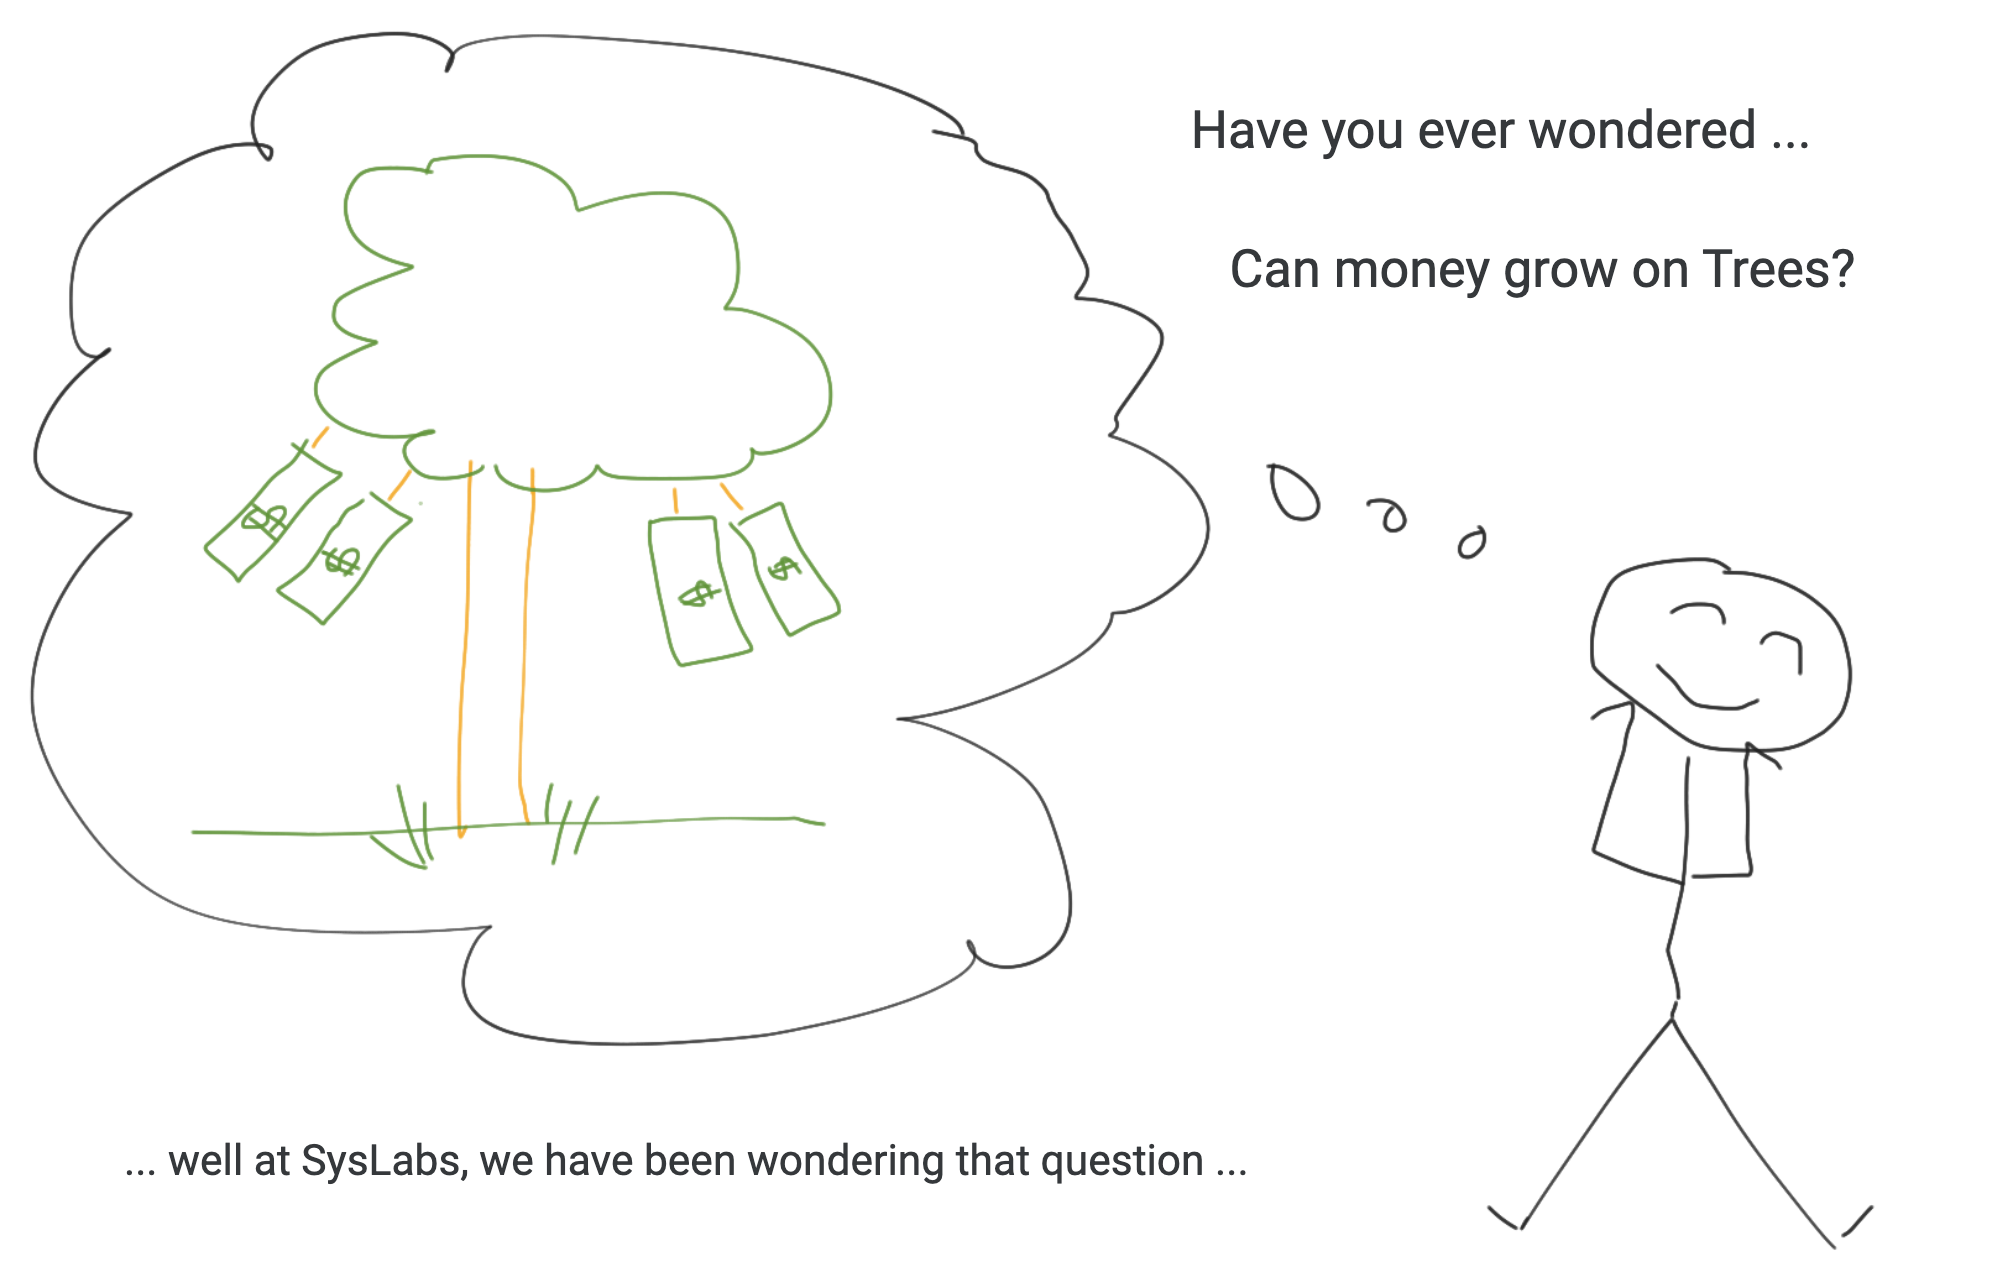
\includegraphics[width=4in]{img/slide1.png}
\label{fig:dex_forest}
\end{figure}
\end{frame}


\begin{frame}{Video: Slide 2}
\begin{figure}[h!]
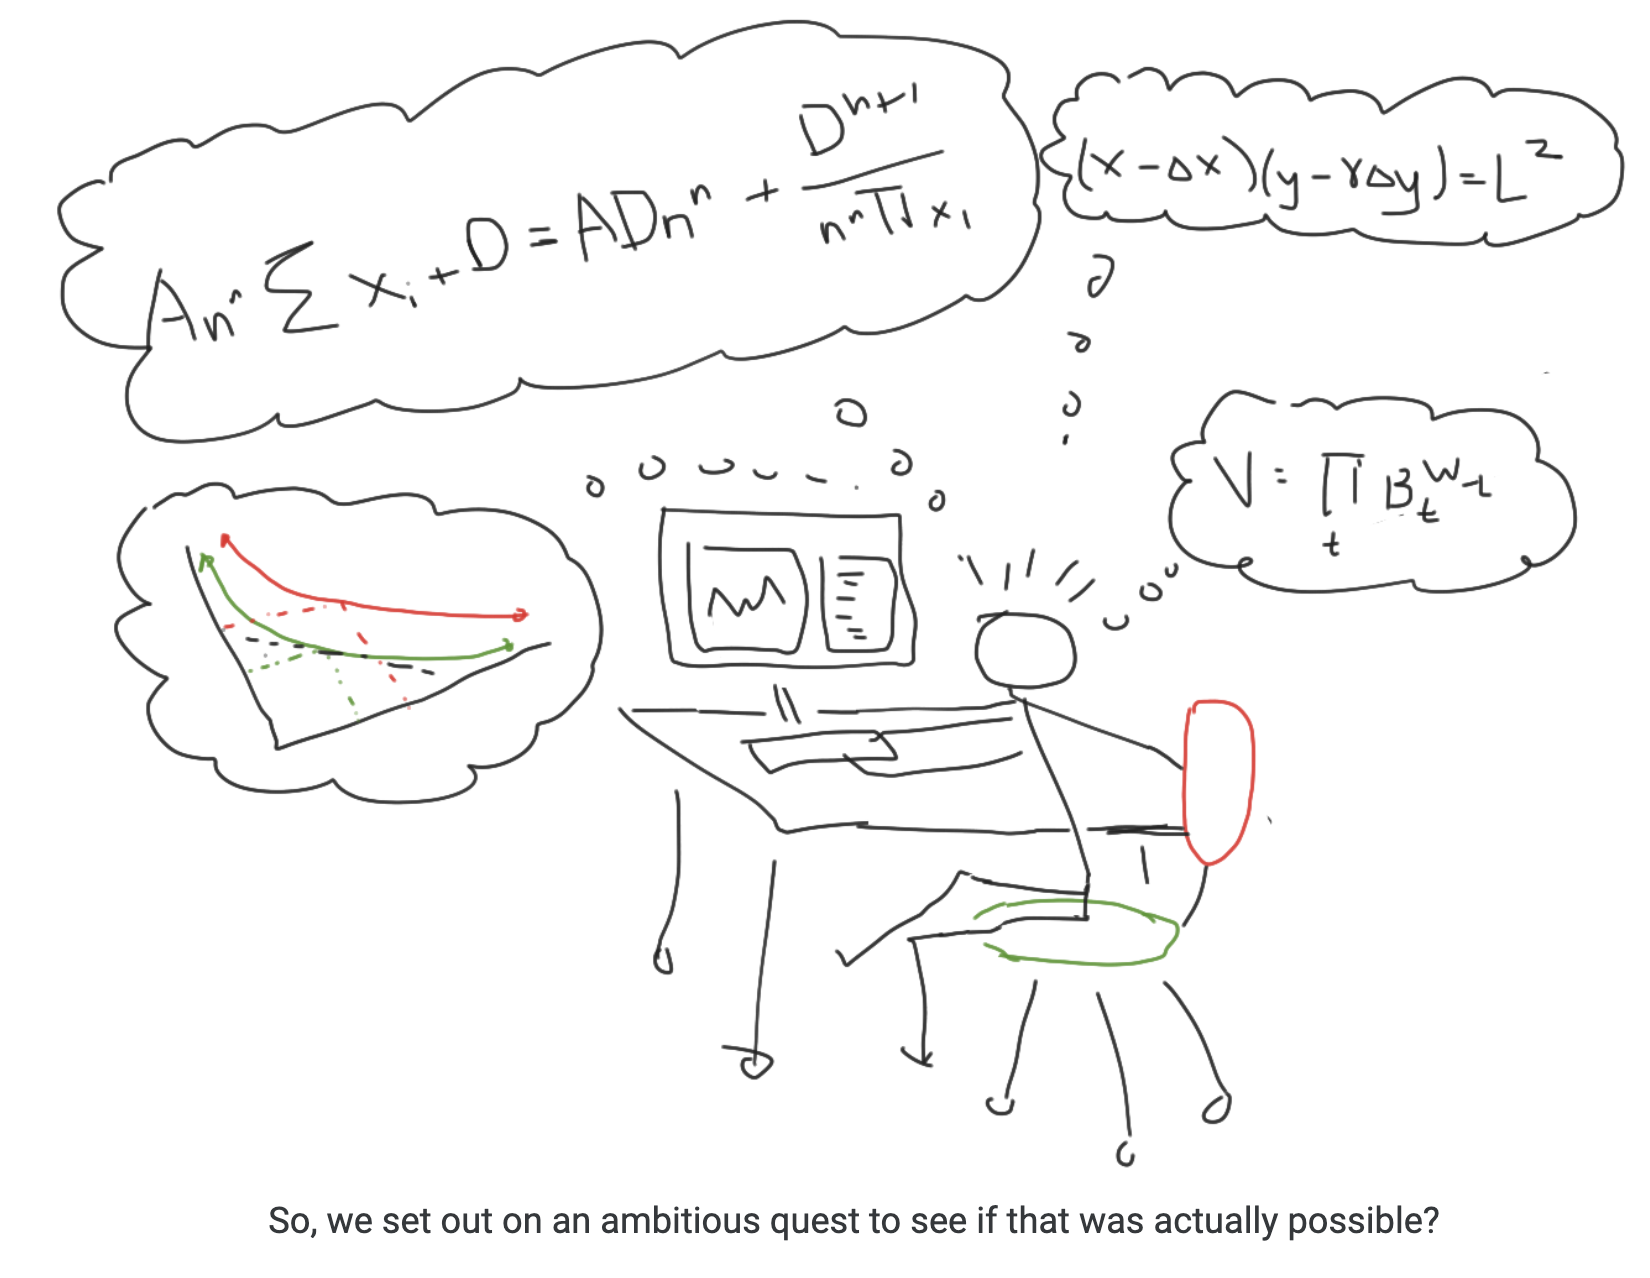
\includegraphics[width=4in]{img/slide2.png}
\label{fig:dex_forest}
\end{figure}
\end{frame}

\begin{frame}{Video: Slide 3}
\begin{figure}[h!]
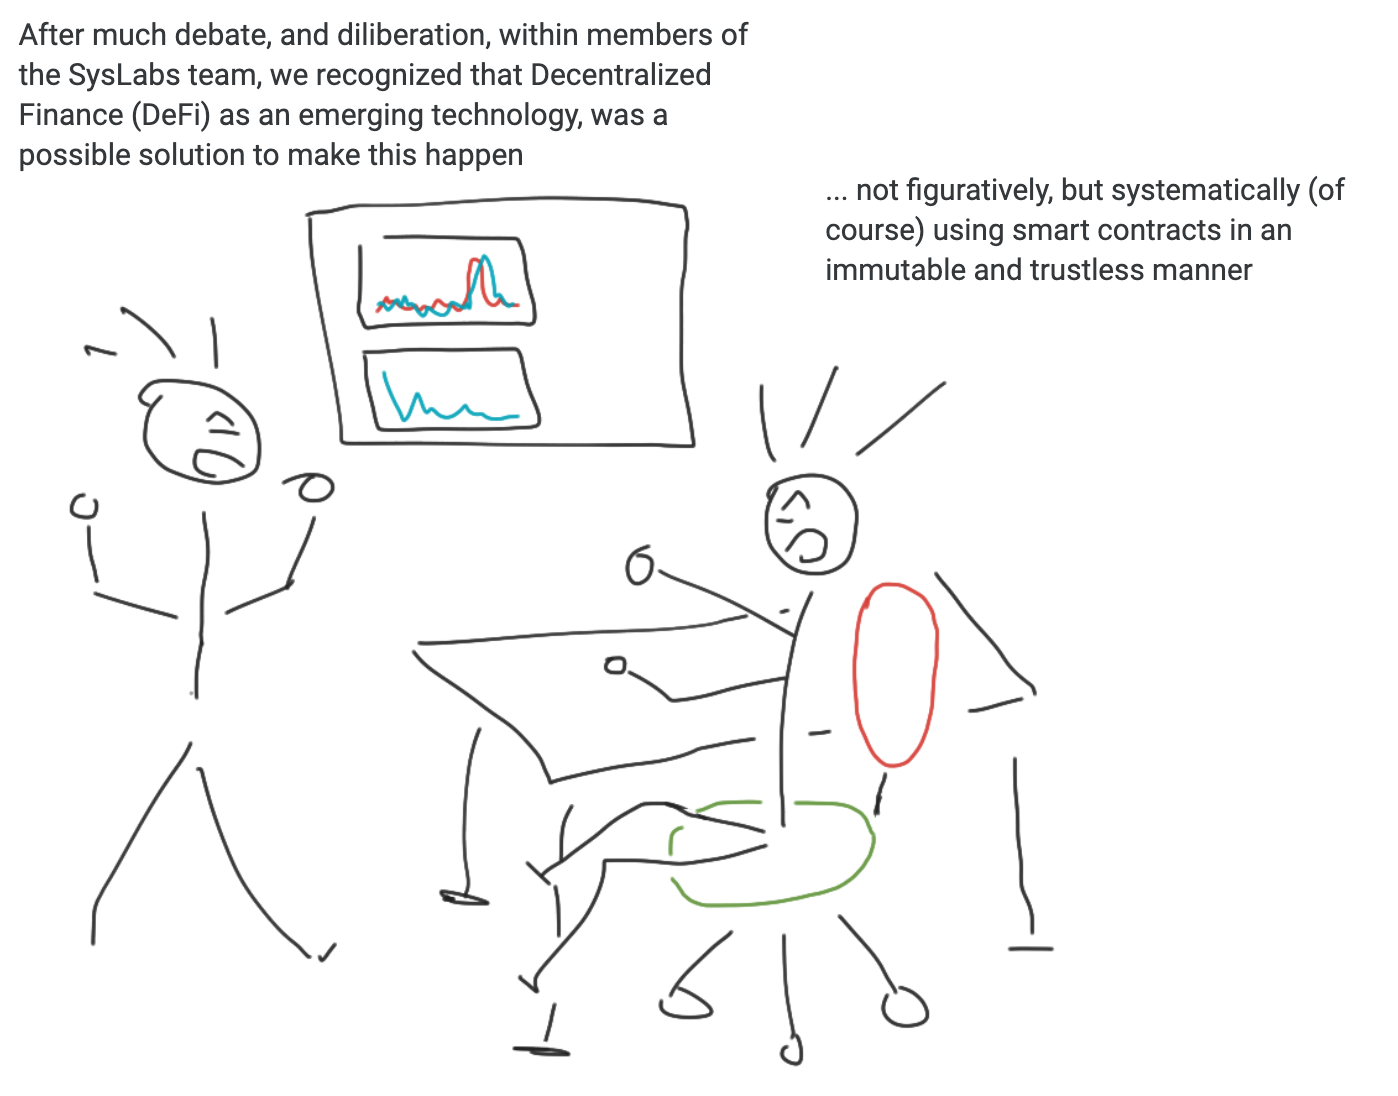
\includegraphics[width=4in]{img/slide3.png}
\label{fig:dex_forest}
\end{figure}
\end{frame}

\begin{frame}{Video: Slide 4}
\begin{figure}[h!]
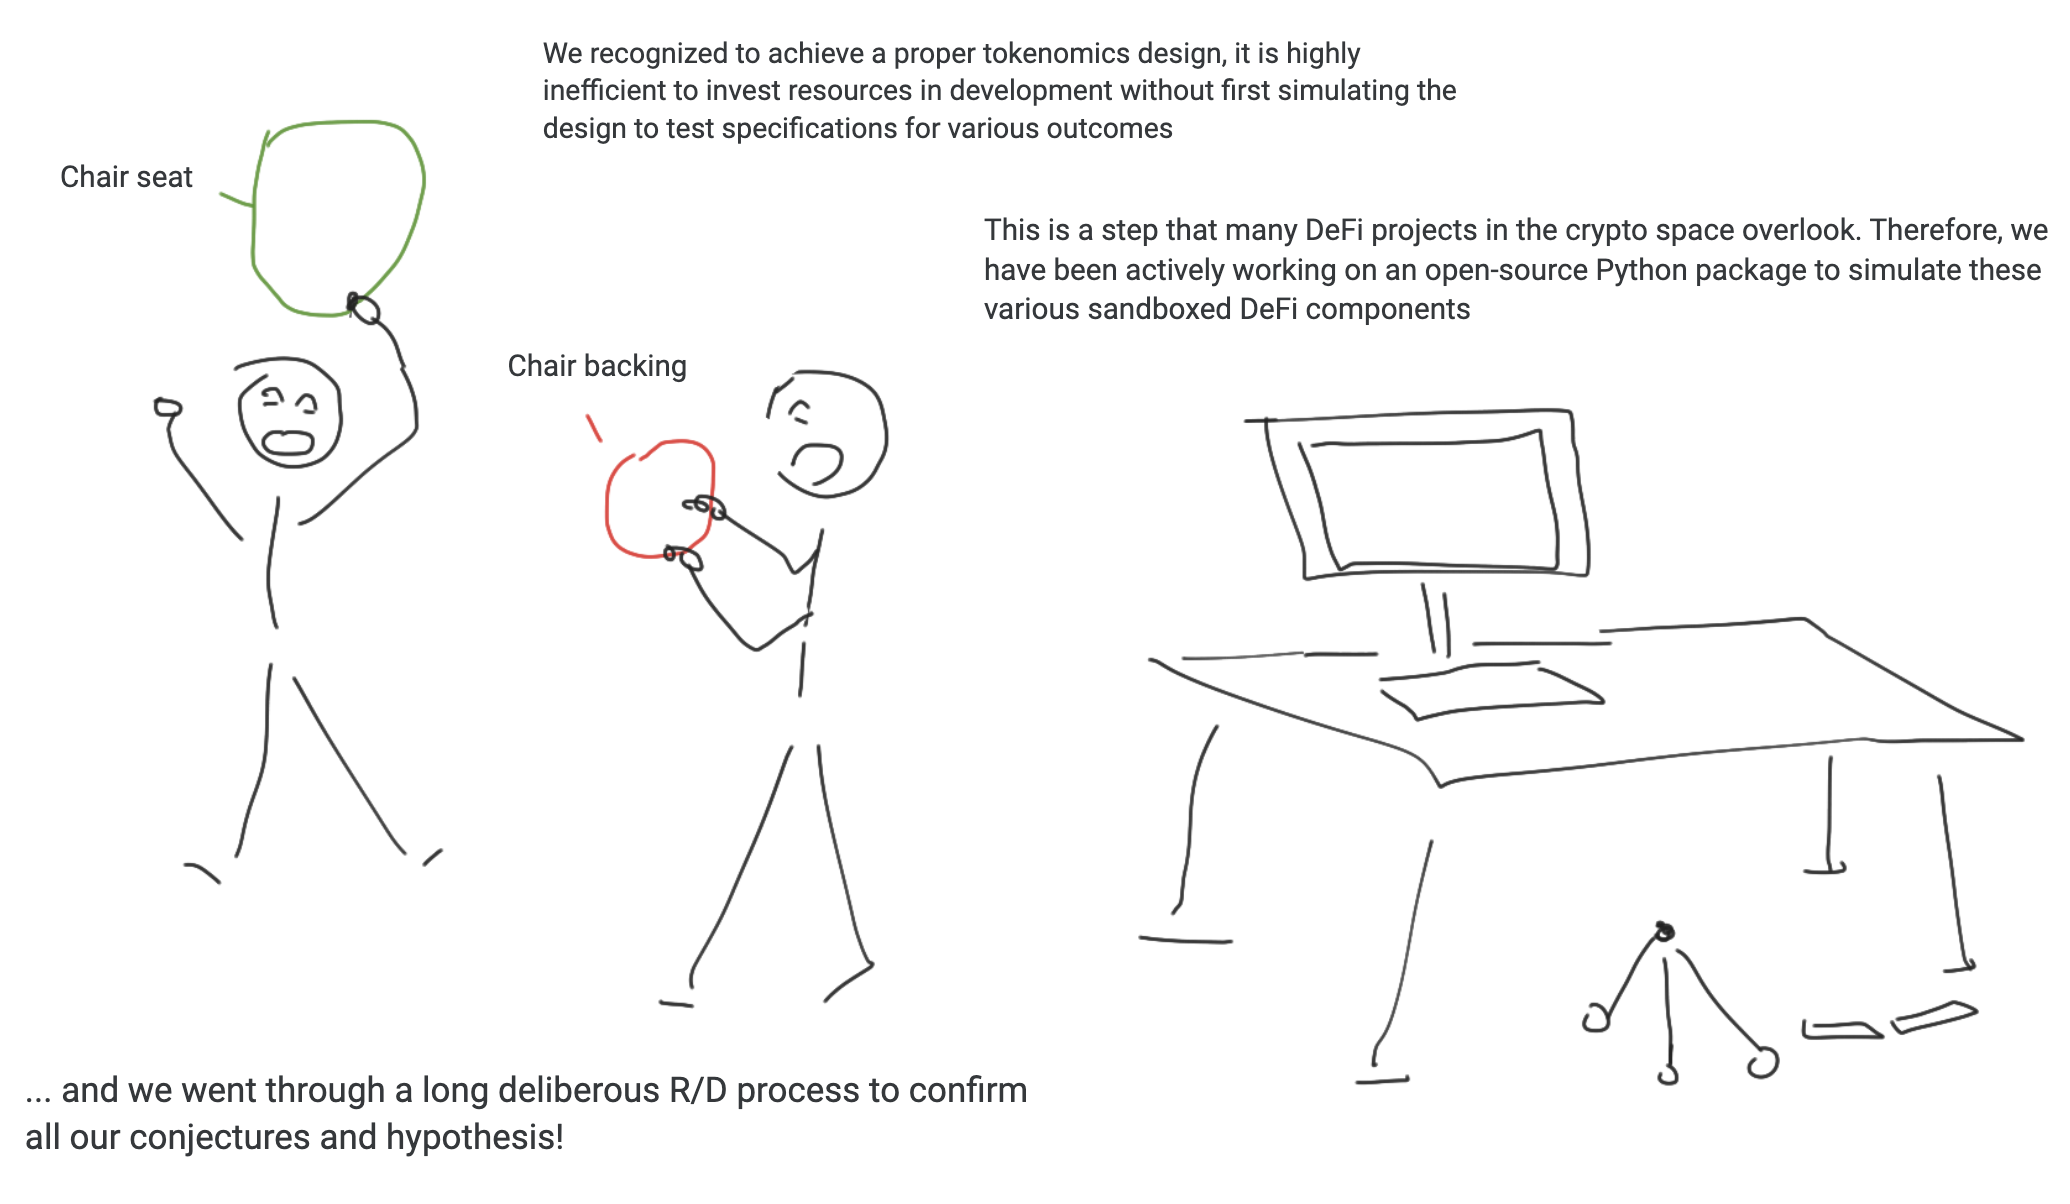
\includegraphics[width=4in]{img/slide4.png}
\label{fig:dex_forest}
\end{figure}
\end{frame}

\begin{frame}{Video: Slide 5}
\begin{figure}[h!]
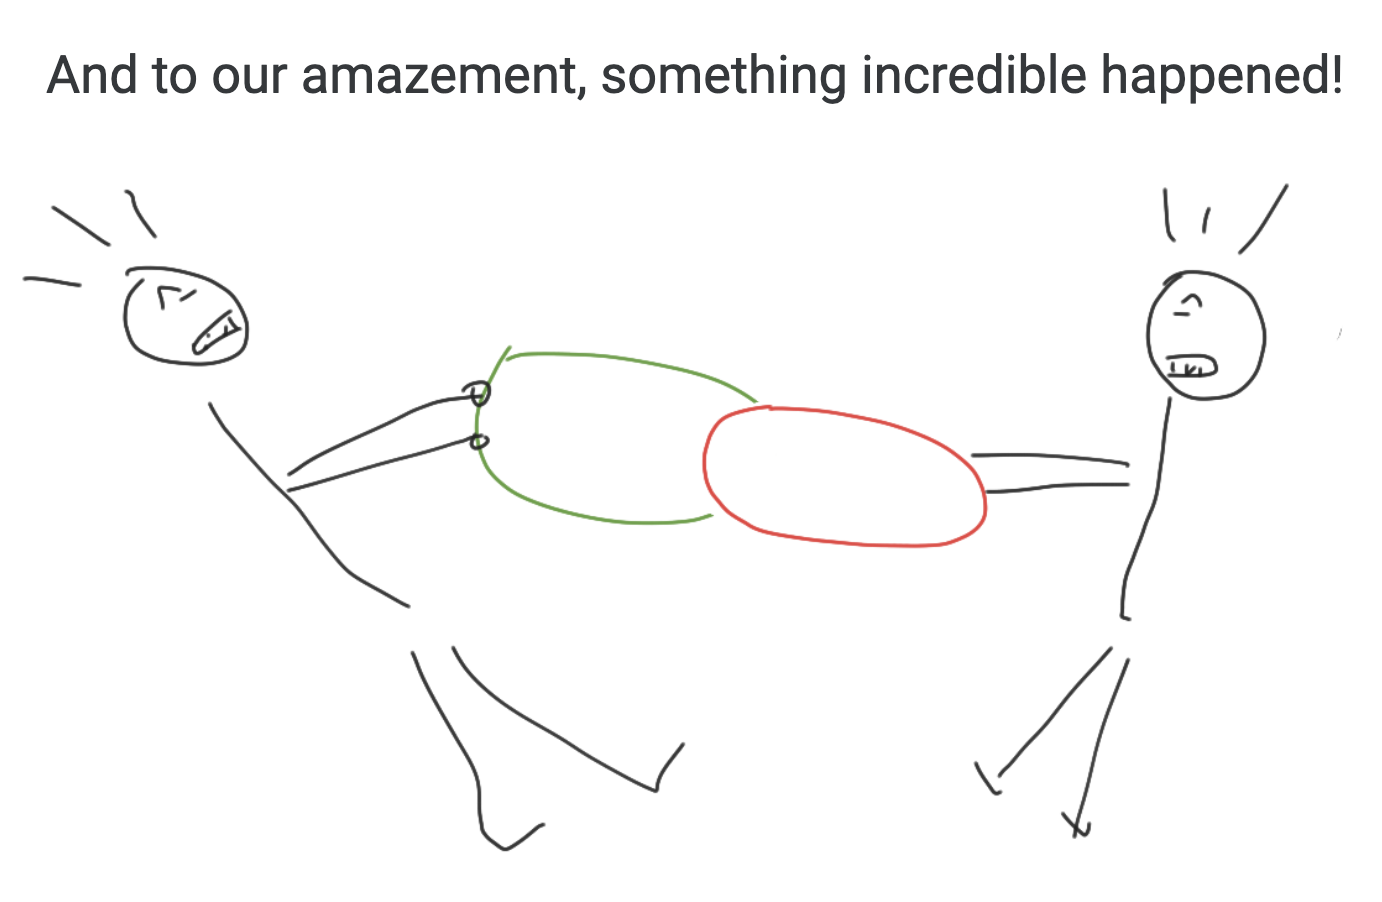
\includegraphics[width=4in]{img/slide5.png}
\label{fig:dex_forest}
\end{figure}
\end{frame}

\begin{frame}{Video: Slide 6}
\begin{figure}[h!]
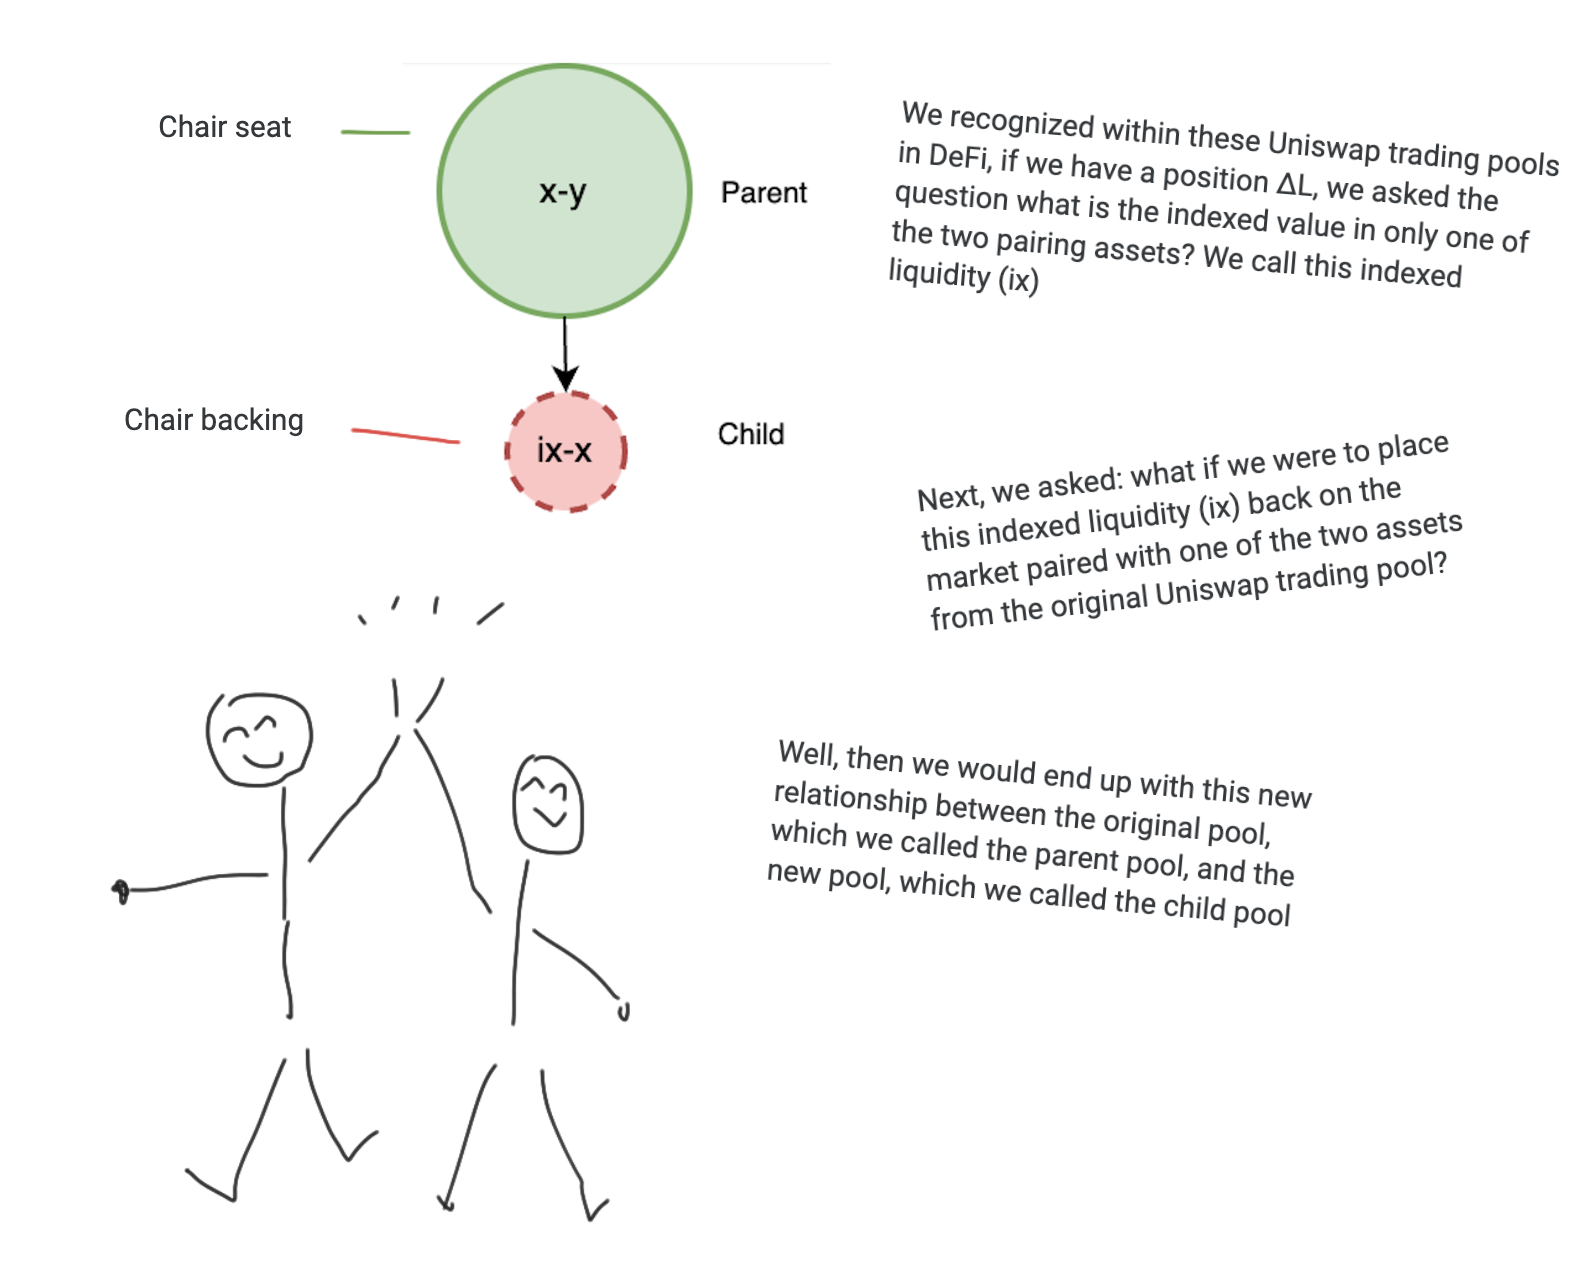
\includegraphics[width=4in]{img/slide6.png}
\label{fig:dex_forest}
\end{figure}
\end{frame}

\begin{frame}{Video: Slide 7}
\begin{figure}[h!]
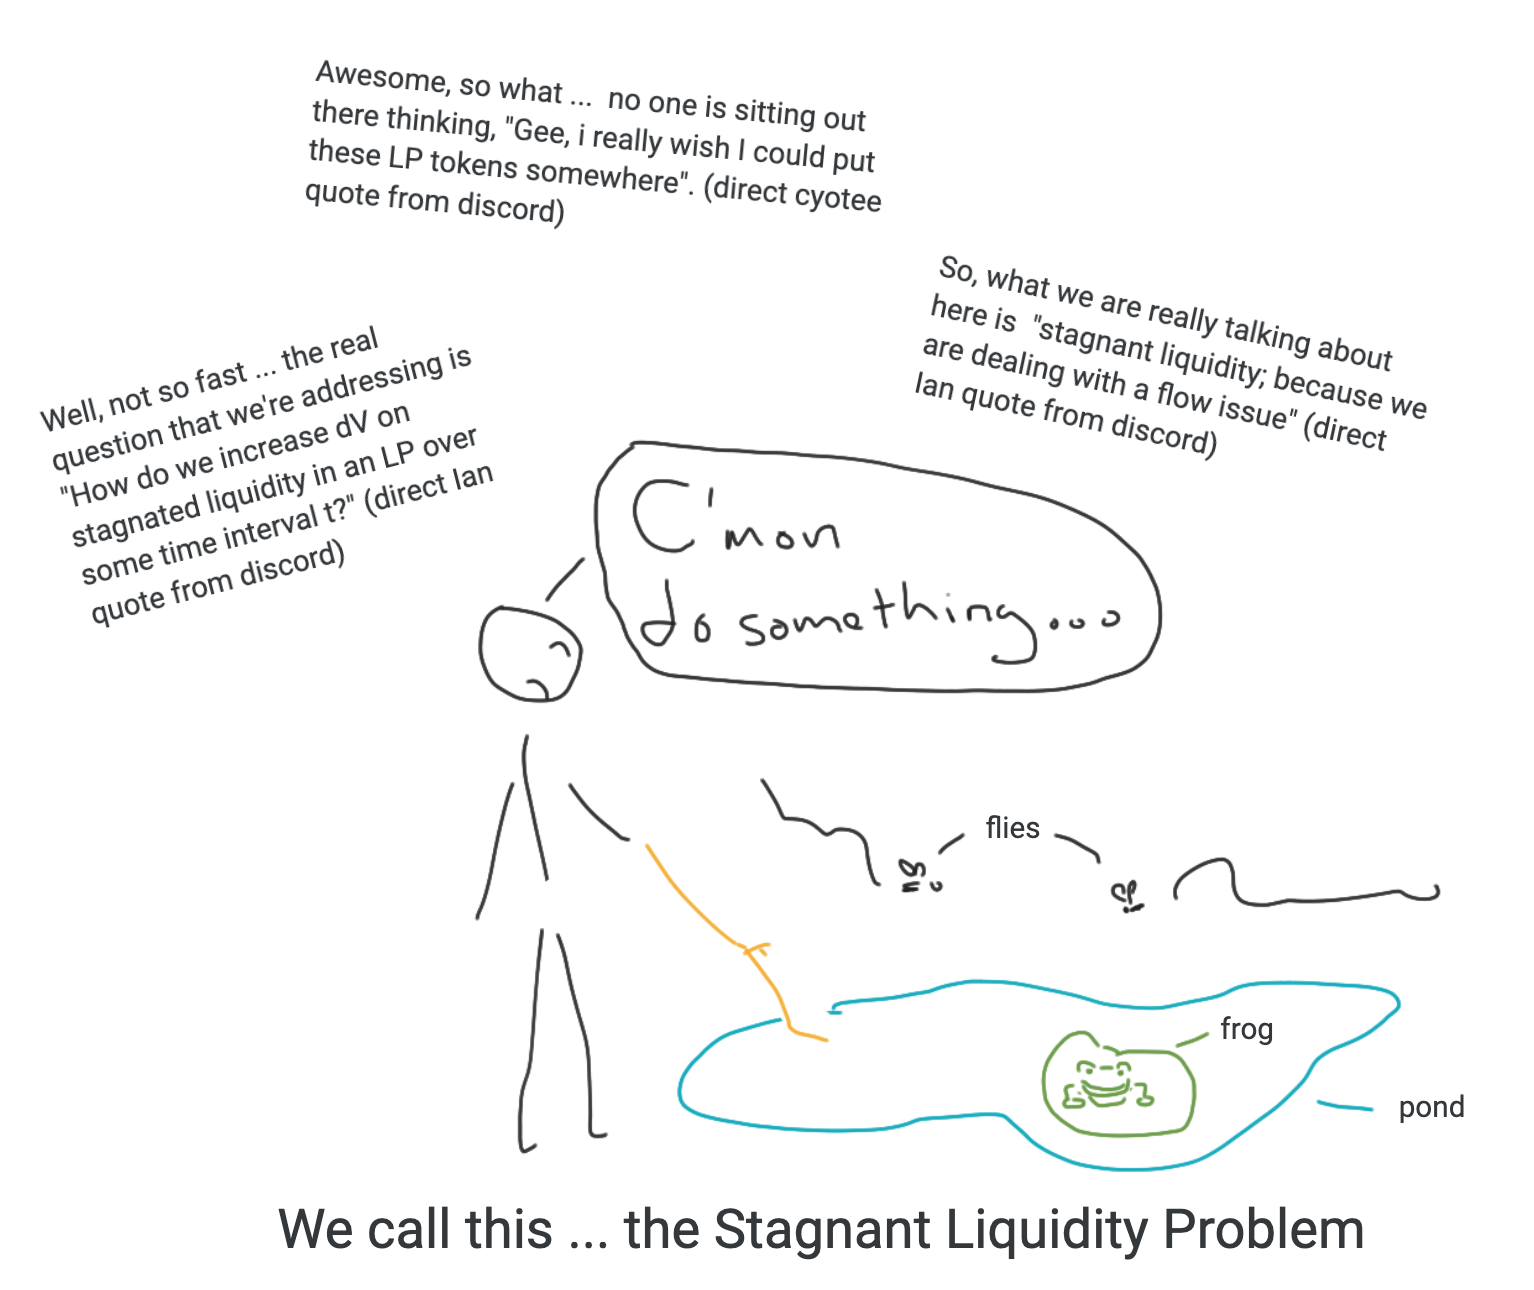
\includegraphics[width=3.6in]{img/slide7.png}
\label{fig:dex_forest}
\end{figure}
\end{frame}

\begin{frame}{Video: Slide 8}
\begin{figure}[h!]
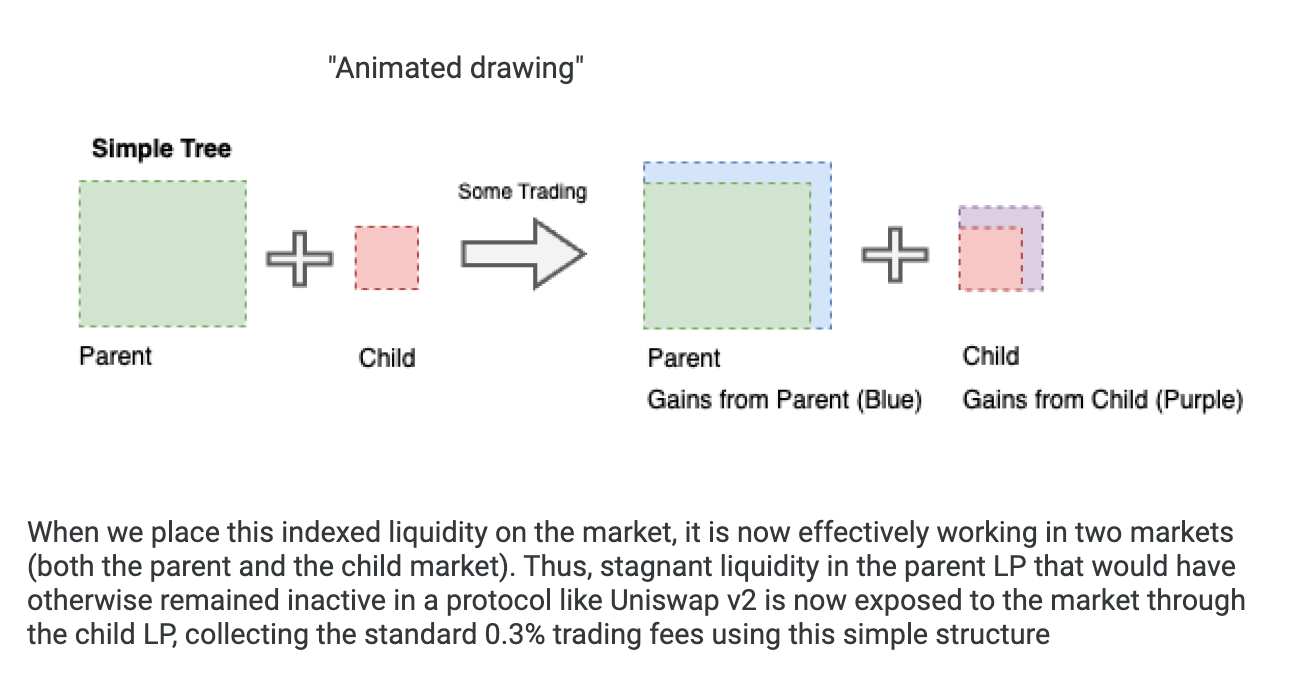
\includegraphics[width=3.6in]{img/slide8.png}
\label{fig:dex_forest}
\end{figure}
\end{frame}

\begin{frame}{Video: Slide 9}
\begin{figure}[h!]
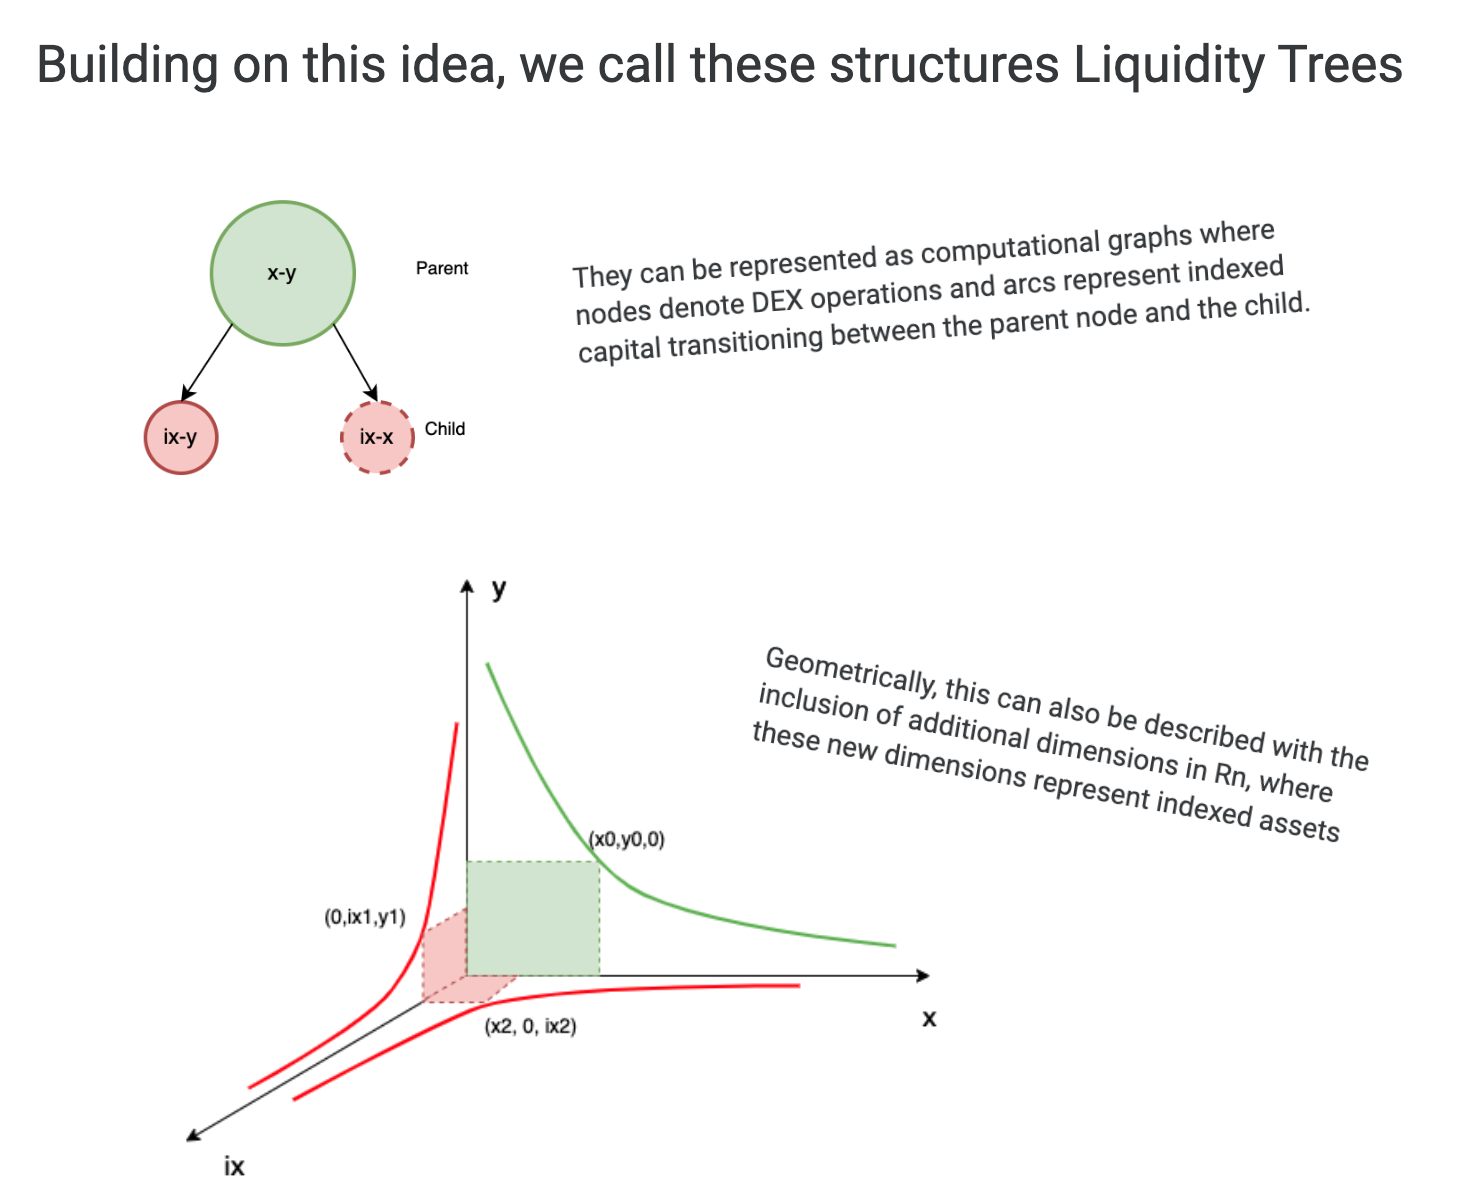
\includegraphics[width=3.6in]{img/slide9.png}
\label{fig:dex_forest}
\end{figure}
\end{frame}

\begin{frame}{Video: Slide 10}
\begin{figure}[h!]
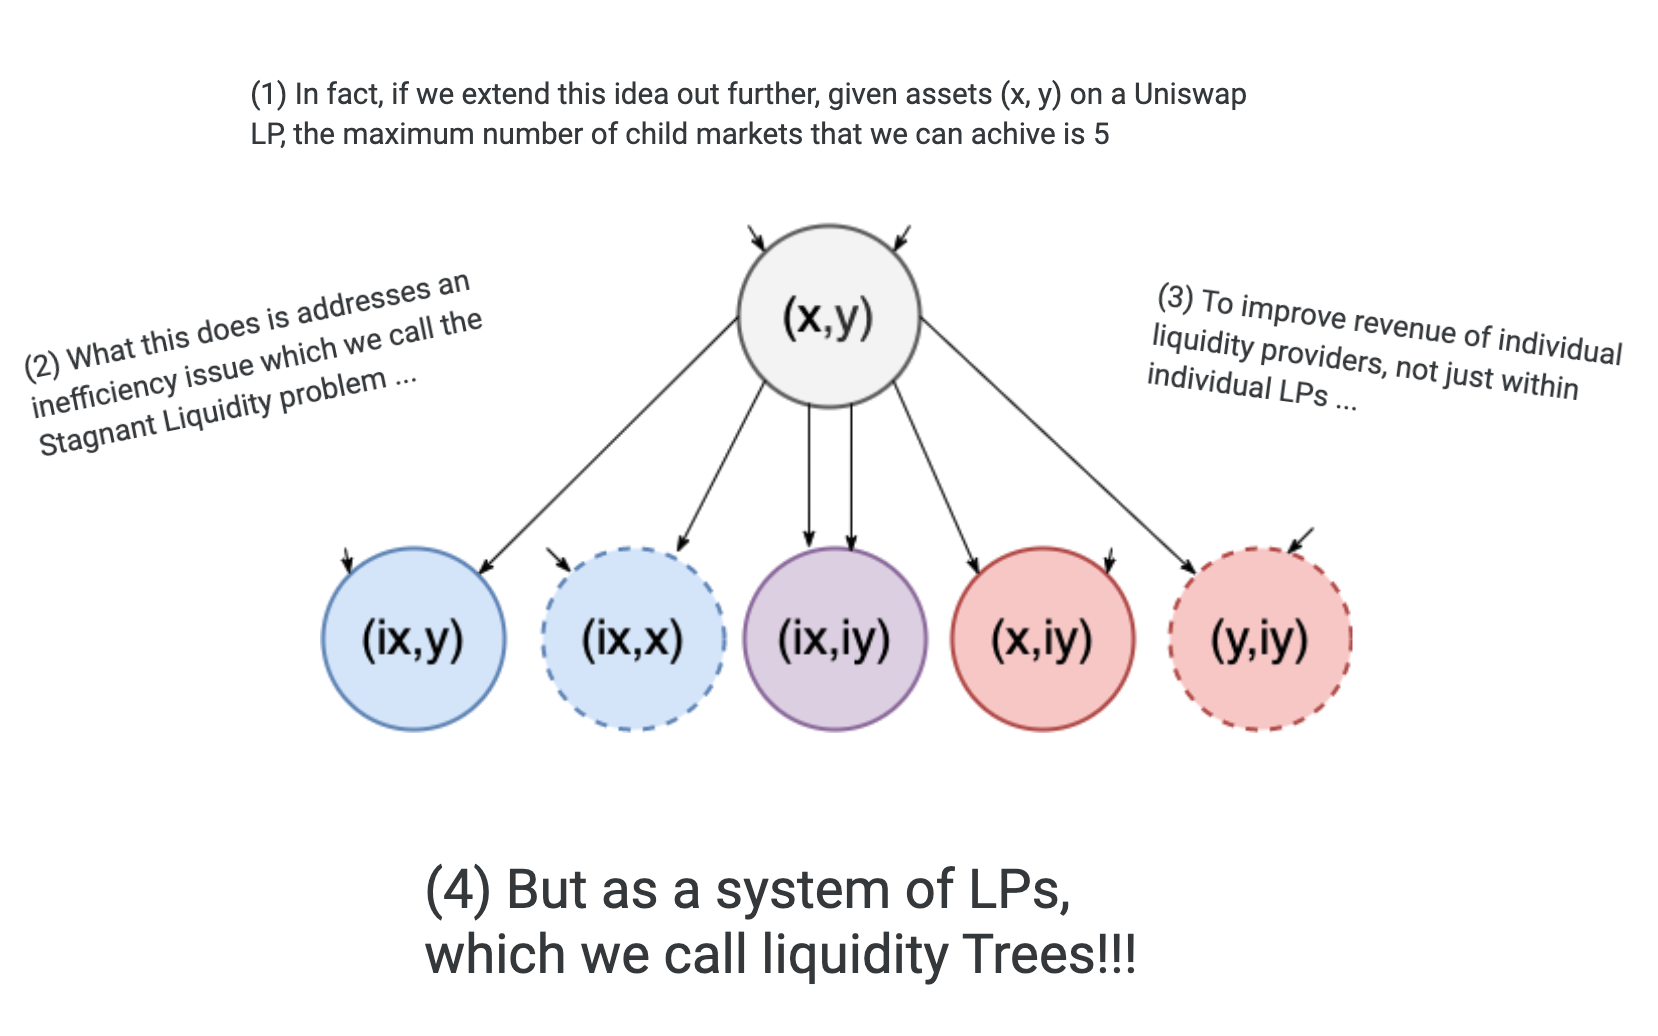
\includegraphics[width=3.6in]{img/slide10.png}
\label{fig:dex_forest}
\end{figure}
\end{frame}

\begin{frame}{Video: Slide 11}
\begin{figure}[h!]
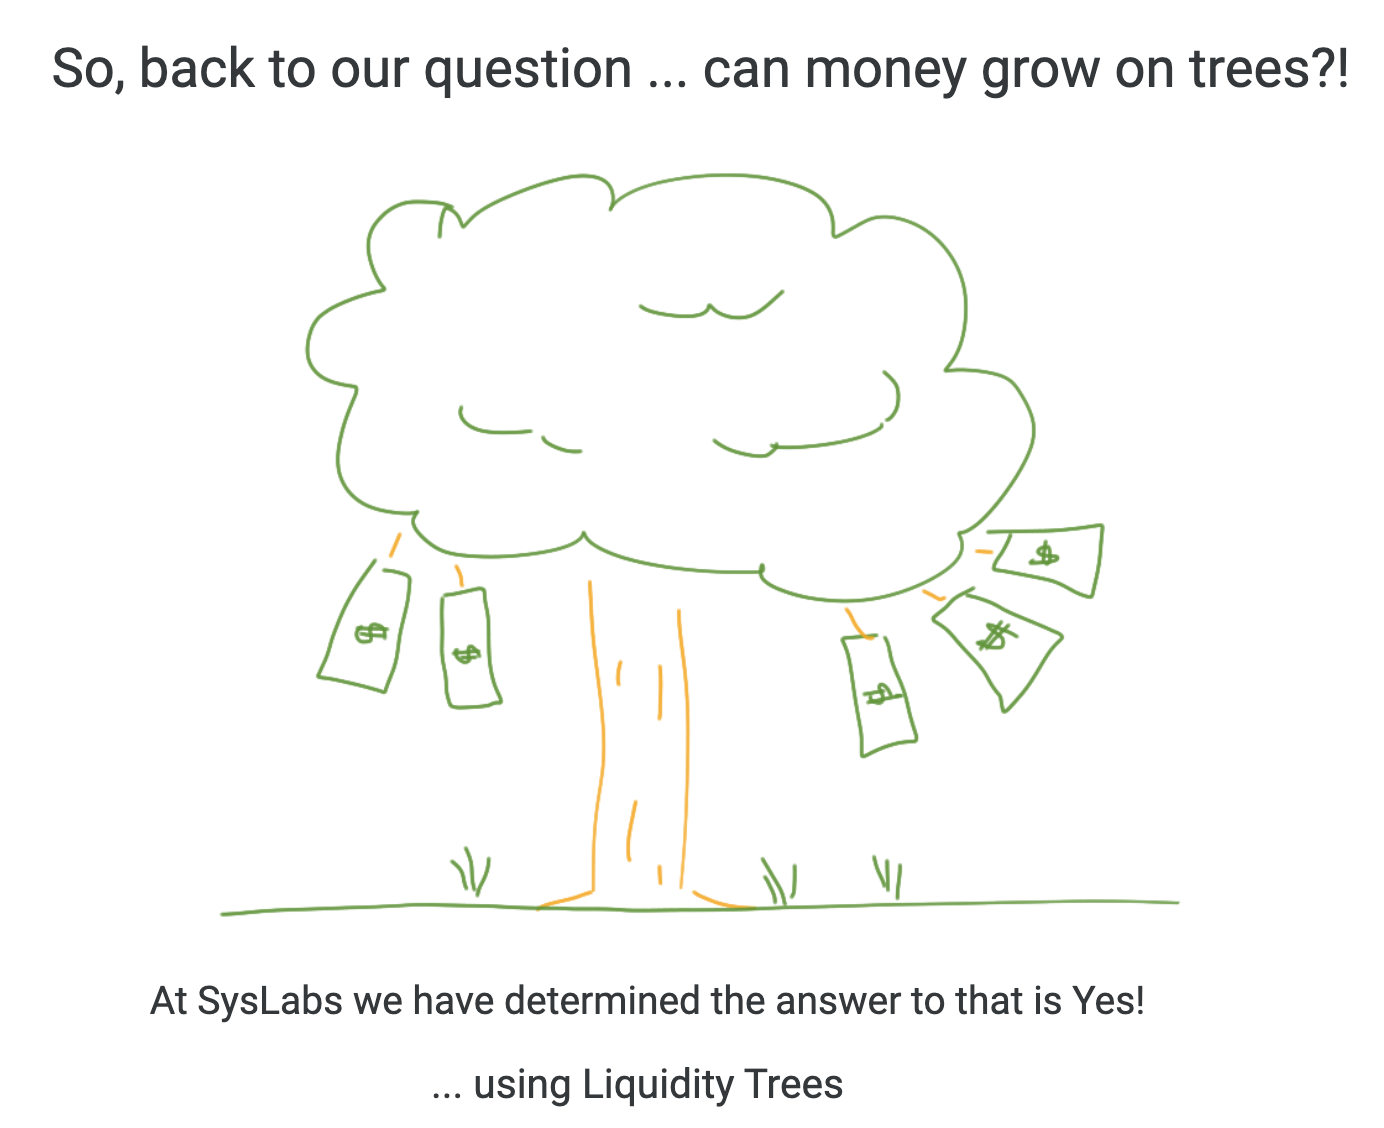
\includegraphics[width=3.6in]{img/slide11.png}
\label{fig:dex_forest}
\end{figure}
\end{frame}

\begin{frame}{Video: Slide 12}
\begin{figure}[h!]
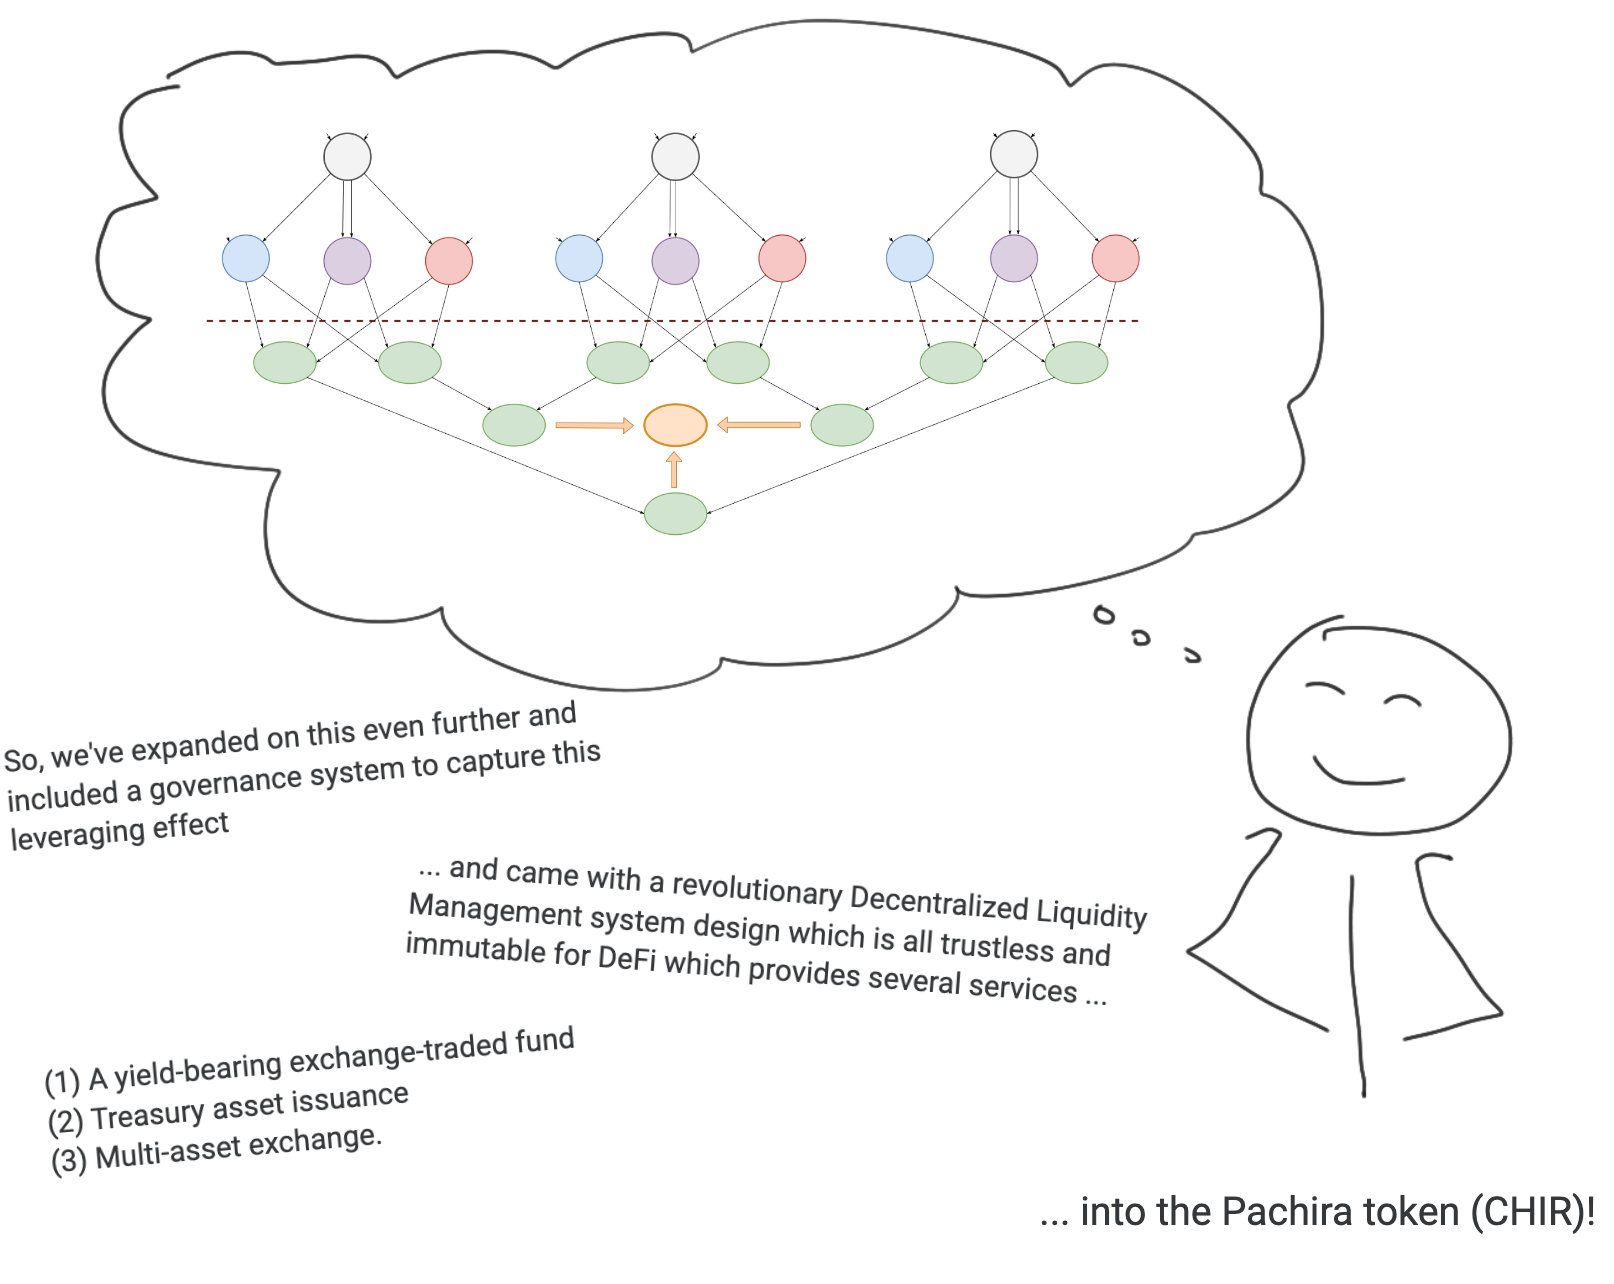
\includegraphics[width=3.6in]{img/slide12.png}
\label{fig:dex_forest}
\end{figure}
\end{frame}


\end{document}